\documentclass[12pt]{article}
\usepackage{tikz}
\usepackage{amsmath}
\usepackage{amsfonts}
\usepackage{geometry}
\usepackage{amssymb}
\usepackage{wasysym}
\usepackage{color}
\usepackage[utf8]{inputenc}
\usepackage{pdfpages}
\usepackage{listings}
\newgeometry{top=1 cm,bottom=2cm,left=0.5cm,right=0.5cm}
\title{ }
\date{}
\author{}


\definecolor{mygreen}{rgb}{0,0.6,0}
\definecolor{mygray}{rgb}{0.5,0.5,0.5}
\definecolor{mymauve}{rgb}{0.58,0,0.82}

\lstset{ %
  backgroundcolor=\color{white},   % choose the background color; you must add \usepackage{color} or \usepackage{xcolor}
  basicstyle=\footnotesize,        % the size of the fonts that are used for the code
  breakatwhitespace=false,         % sets if automatic breaks should only happen at whitespace
  breaklines=true,                 % sets automatic line breaking
  captionpos=b,                    % sets the caption-position to bottom
  commentstyle=\color{mygreen},    % comment style
  deletekeywords={...},            % if you want to delete keywords from the given language
  escapeinside={\%*}{*)},          % if you want to add LaTeX within your code
  extendedchars=true,              % lets you use non-ASCII characters; for 8-bits encodings only, does not work with UTF-8
  frame=single,	                   % adds a frame around the code
  keepspaces=true,                 % keeps spaces in text, useful for keeping indentation of code (possibly needs columns=flexible)
  keywordstyle=\color{blue},       % keyword style
  language=Octave,                 % the language of the code
  otherkeywords={*,...},           % if you want to add more keywords to the set
  numbers=left,                    % where to put the line-numbers; possible values are (none, left, right)
  numbersep=5pt,                   % how far the line-numbers are from the code
  numberstyle=\tiny\color{mygray}, % the style that is used for the line-numbers
  rulecolor=\color{black},         % if not set, the frame-color may be changed on line-breaks within not-black text (e.g. comments (green here))
  showspaces=false,                % show spaces everywhere adding particular underscores; it overrides 'showstringspaces'
  showstringspaces=false,          % underline spaces within strings only
  showtabs=false,                  % show tabs within strings adding particular underscores
  stepnumber=2,                    % the step between two line-numbers. If it's 1, each line will be numbered
  stringstyle=\color{mymauve},     % string literal style
  tabsize=2,	                   % sets default tabsize to 2 spaces
  title=\lstname,                  % show the filename of files included with \lstinputlisting; also try caption instead of title
  xleftmargin=0cm,
}

\title{Graphs with large minimum vertex energy}
\date{}
\author{}
\begin{document}

\noindent Problema: Sea $G$ una gráfica conexa , demuestre que existe una trayectoria de tamaño $\min(2\delta,n-1)$.\\

\noindent Solución:\\

\noindent Supondremos que $\delta \geq 2$ pues si $\delta=1$ la gráfica es $K_2$ y es trivial.\\

\noindent Lo haremos por contradicción, supongamos que no, sea $P=x_1,x_2,\dots, x_m$ una trayectoria de longitud máxima, con $m\leq \min(2\delta,n-1)$. Es claro que todos los vecinos de $x_1$ y $x_m$ están en $P$. Supongamos que para cada vecino $x_k$ de $x_m$  se cumple que $x_{k+1}$ no es vecino de $x_1$. Entonces $x_1$ tiene a lo más $(m-1)-\deg(x_n)$ vecinos. Concluimos que $\deg(x_1)+\deg(x_m)\leq m-1< 2 \delta$, una contradicción. Por lo tanto existe un ciclo $C$ con la misma longitud que $P$ ( explicitamente es el ciclo $x_1,x_2,\dots,x_k,x_n,x_{n-1},\dots,x_{k+1},x_1$).\\

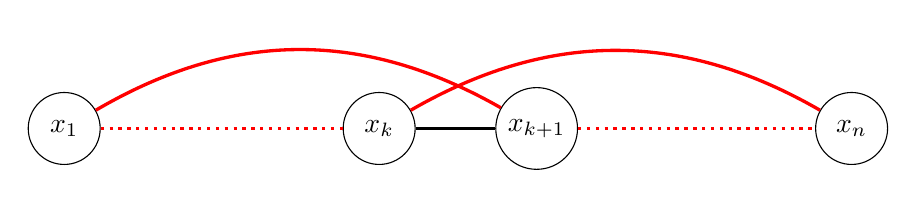
\begin{tikzpicture}
\node[style={circle,fill=white,draw,minimum size=2.6em,inner sep=3pt]}] (1) at (2,0) {$x_1$};
\node[style={circle,fill=white,draw,minimum size=2.6em,inner sep=3pt]}] (3) at (6,0) {$x_k$};
\node[style={circle,fill=white,draw,minimum size=2.6em,inner sep=3pt]}] (4) at (8,0) {$x_{k+1}$};
\node[style={circle,fill=white,draw,minimum size=2.6em,inner sep=3pt]}] (5) at (12,0) {$x_n$};
\path[draw,very thick,red,dotted](1) edge node {} (3);
\path[draw,very thick](3) edge node {} (4);
\path[draw,very thick,red,dotted](4) edge node {} (5);
\path[draw,very thick,red](3) edge[bend left] node {} (5);
\path[draw,very thick,red](1) edge[bend left] node {} (4);
\end{tikzpicture}



\noindent Por hipótesis tenemos que $C$ no contiene todos los vértices de $G$, como $G$ es conexa existe un vértice de $C$ conectado a un vértice  fuera de $C$. Esto es una contradicción, pues nos permite construir una trayectoria más grande que $P$.\\

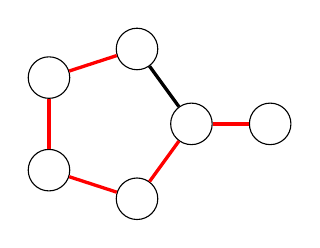
\begin{tikzpicture}
\node[style={circle,fill=white,draw,minimum size=1.5em,inner sep=3pt]}] (1) at (1*360/5:1) {};
\node[style={circle,fill=white,draw,minimum size=1.5em,inner sep=3pt]}] (2) at (2*360/5:1) {};
\node[style={circle,fill=white,draw,minimum size=1.5em,inner sep=3pt]}] (3) at (3*360/5:1) {};
\node[style={circle,fill=white,draw,minimum size=1.5em,inner sep=3pt]}] (4) at (4*360/5:1) {};
\node[style={circle,fill=white,draw,minimum size=1.5em,inner sep=3pt]}] (5) at (5*360/5:1) {};
\node[style={circle,fill=white,draw,minimum size=1.5em,inner sep=3pt]}] (6) at (5*360/5:2) {};
\path[draw,very thick,red](1) edge node {} (2);
\path[draw,very thick](1) edge node {} (5);
\path[draw,very thick,red](2) edge node {} (3);
\path[draw,very thick,red](3) edge node {} (4);
\path[draw,very thick,red](4) edge node {} (5);
\path[draw,very thick,red](5) edge node {} (6);
\end{tikzpicture}





\end{document}